% backtracking worksheet template
\documentclass[leqno, 12pt]{article}
\usepackage{tikz}
\usetikzlibrary{positioning}
\usetikzlibrary {arrows.meta}
\usepackage[a4paper, portrait, margin=1cm]{geometry}
\usepackage{multicol}
\usepackage{fancyhdr}

\tikzset{backtrack/.style={rectangle,draw=black,fill=white,
inner sep=2pt,minimum height=32pt, minimum width=20mm}}
\tikzset{backtrackeq/.style={rectangle,draw=black,fill=white,
inner sep=2pt,minimum height=12pt, minimum width=20mm}}
\tikzset{backtrackstep/.style={rectangle,draw=none,fill=white,
inner sep=2pt,minimum height=12pt, minimum width=20mm}}

\def \HeadingAnswers {\section*{\Large Name: \underline{\hspace{8cm}} \hfill Date: \underline{\hspace{3cm}}} \vspace{-3mm}
{2-step backtracking: Answers} \vspace{1pt}\hrule}

% raise footer with page number; no header
\fancypagestyle{myfancypagestyle}{
  \fancyhf{}% clear all header and footer fields
  \renewcommand{\headrulewidth}{0pt} % no rule under header
  \fancyfoot[C] {\thepage} \setlength{\footskip}{14.5pt} % raise page number allowed min 14.5pt
}
\pagestyle{myfancypagestyle}  % apply myfancypagestyle

\begin{document}
    \HeadingAnswers
    \vspace{-8mm}
    \begin{multicols}{2}
        \begin{equation}
    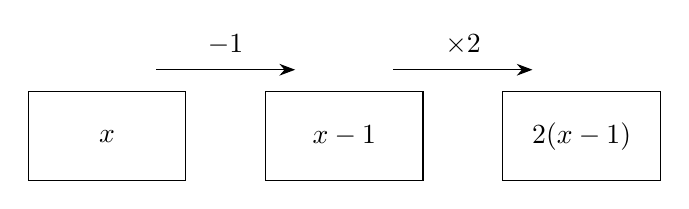
\begin{tikzpicture}[baseline={([yshift=-12pt]current bounding box.north)}]

        \node[backtrack] (boxA) at (0, 0) {$x$};
        \node[backtrack] (boxB) [right=1cm of boxA] {$x-1$};
        \node[backtrack] (boxC) [right=1cm of boxB] {$2(x-1)$};

        \node (boxAr) at ([yshift=24pt,xshift=5mm]boxA) { };
        \node (boxBl) at ([yshift=24pt,xshift=-5mm]boxB) { };
        \draw [line width=0.4pt,-{Stealth[length=2mm]}] (boxAr)  --node[backtrackstep, above=3.0pt] {$-1$} (boxBl);

        \node (boxBr) at ([yshift=24pt,xshift=5mm]boxB) { };
        \node (boxCl) at ([yshift=24pt,xshift=-5mm]boxC) { };
        \draw [line width=0.4pt,-{Stealth[length=2mm]}] (boxBr)  --node[backtrackstep, above=3.0pt] {$\times2$} (boxCl);

    \end{tikzpicture}
\end{equation}


\vspace{-2pt}\begin{equation}
    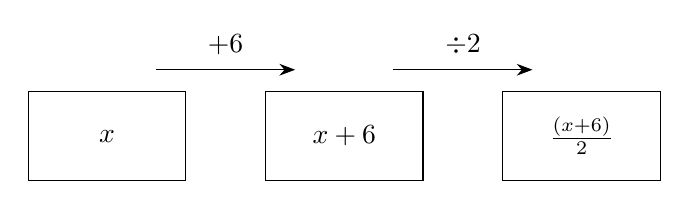
\begin{tikzpicture}[baseline={([yshift=-12pt]current bounding box.north)}]

        \node[backtrack] (boxA) at (0, 0) {$x$};
        \node[backtrack] (boxB) [right=1cm of boxA] {$x+6$};
        \node[backtrack] (boxC) [right=1cm of boxB] {$\frac{(x+6)}{2}$};

        \node (boxAr) at ([yshift=24pt,xshift=5mm]boxA) { };
        \node (boxBl) at ([yshift=24pt,xshift=-5mm]boxB) { };
        \draw [line width=0.4pt,-{Stealth[length=2mm]}] (boxAr)  --node[backtrackstep, above=3.0pt] {$+6$} (boxBl);

        \node (boxBr) at ([yshift=24pt,xshift=5mm]boxB) { };
        \node (boxCl) at ([yshift=24pt,xshift=-5mm]boxC) { };
        \draw [line width=0.4pt,-{Stealth[length=2mm]}] (boxBr)  --node[backtrackstep, above=3.0pt] {$\div2$} (boxCl);

    \end{tikzpicture}
\end{equation}


\vspace{-2pt}\begin{equation}
    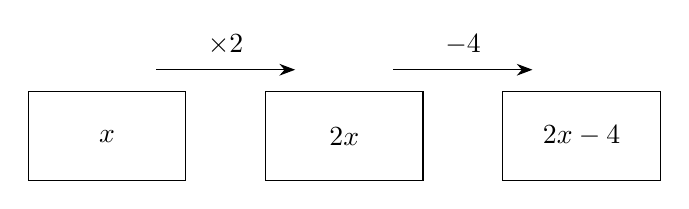
\begin{tikzpicture}[baseline={([yshift=-12pt]current bounding box.north)}]

        \node[backtrack] (boxA) at (0, 0) {$x$};
        \node[backtrack] (boxB) [right=1cm of boxA] {$2x$};
        \node[backtrack] (boxC) [right=1cm of boxB] {$2x - 4$};

        \node (boxAr) at ([yshift=24pt,xshift=5mm]boxA) { };
        \node (boxBl) at ([yshift=24pt,xshift=-5mm]boxB) { };
        \draw [line width=0.4pt,-{Stealth[length=2mm]}] (boxAr)  --node[backtrackstep, above=3.0pt] {$\times2$} (boxBl);

        \node (boxBr) at ([yshift=24pt,xshift=5mm]boxB) { };
        \node (boxCl) at ([yshift=24pt,xshift=-5mm]boxC) { };
        \draw [line width=0.4pt,-{Stealth[length=2mm]}] (boxBr)  --node[backtrackstep, above=3.0pt] {$-4$} (boxCl);

    \end{tikzpicture}
\end{equation}


\vspace{-2pt}\begin{equation}
    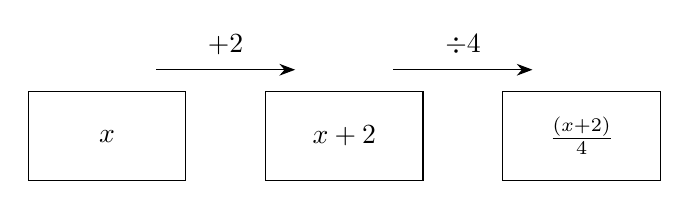
\begin{tikzpicture}[baseline={([yshift=-12pt]current bounding box.north)}]

        \node[backtrack] (boxA) at (0, 0) {$x$};
        \node[backtrack] (boxB) [right=1cm of boxA] {$x+2$};
        \node[backtrack] (boxC) [right=1cm of boxB] {$\frac{(x+2)}{4}$};

        \node (boxAr) at ([yshift=24pt,xshift=5mm]boxA) { };
        \node (boxBl) at ([yshift=24pt,xshift=-5mm]boxB) { };
        \draw [line width=0.4pt,-{Stealth[length=2mm]}] (boxAr)  --node[backtrackstep, above=3.0pt] {$+2$} (boxBl);

        \node (boxBr) at ([yshift=24pt,xshift=5mm]boxB) { };
        \node (boxCl) at ([yshift=24pt,xshift=-5mm]boxC) { };
        \draw [line width=0.4pt,-{Stealth[length=2mm]}] (boxBr)  --node[backtrackstep, above=3.0pt] {$\div4$} (boxCl);

    \end{tikzpicture}
\end{equation}


\vspace{-2pt}\begin{equation}
    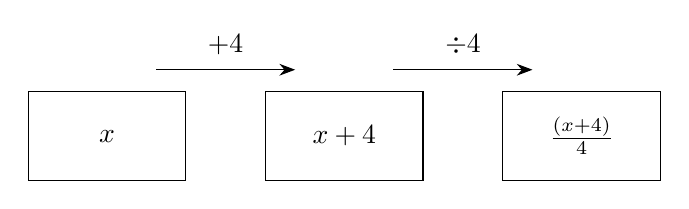
\begin{tikzpicture}[baseline={([yshift=-12pt]current bounding box.north)}]

        \node[backtrack] (boxA) at (0, 0) {$x$};
        \node[backtrack] (boxB) [right=1cm of boxA] {$x+4$};
        \node[backtrack] (boxC) [right=1cm of boxB] {$\frac{(x+4)}{4}$};

        \node (boxAr) at ([yshift=24pt,xshift=5mm]boxA) { };
        \node (boxBl) at ([yshift=24pt,xshift=-5mm]boxB) { };
        \draw [line width=0.4pt,-{Stealth[length=2mm]}] (boxAr)  --node[backtrackstep, above=3.0pt] {$+4$} (boxBl);

        \node (boxBr) at ([yshift=24pt,xshift=5mm]boxB) { };
        \node (boxCl) at ([yshift=24pt,xshift=-5mm]boxC) { };
        \draw [line width=0.4pt,-{Stealth[length=2mm]}] (boxBr)  --node[backtrackstep, above=3.0pt] {$\div4$} (boxCl);

    \end{tikzpicture}
\end{equation}


\vspace{-2pt}\begin{equation}
    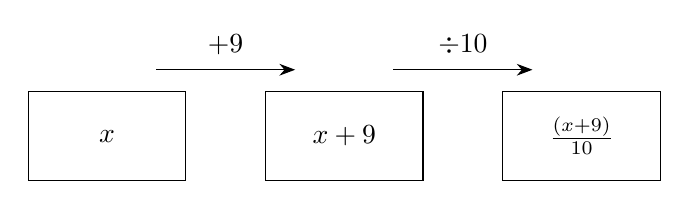
\begin{tikzpicture}[baseline={([yshift=-12pt]current bounding box.north)}]

        \node[backtrack] (boxA) at (0, 0) {$x$};
        \node[backtrack] (boxB) [right=1cm of boxA] {$x+9$};
        \node[backtrack] (boxC) [right=1cm of boxB] {$\frac{(x+9)}{10}$};

        \node (boxAr) at ([yshift=24pt,xshift=5mm]boxA) { };
        \node (boxBl) at ([yshift=24pt,xshift=-5mm]boxB) { };
        \draw [line width=0.4pt,-{Stealth[length=2mm]}] (boxAr)  --node[backtrackstep, above=3.0pt] {$+9$} (boxBl);

        \node (boxBr) at ([yshift=24pt,xshift=5mm]boxB) { };
        \node (boxCl) at ([yshift=24pt,xshift=-5mm]boxC) { };
        \draw [line width=0.4pt,-{Stealth[length=2mm]}] (boxBr)  --node[backtrackstep, above=3.0pt] {$\div10$} (boxCl);

    \end{tikzpicture}
\end{equation}


\vspace{-2pt}\begin{equation}
    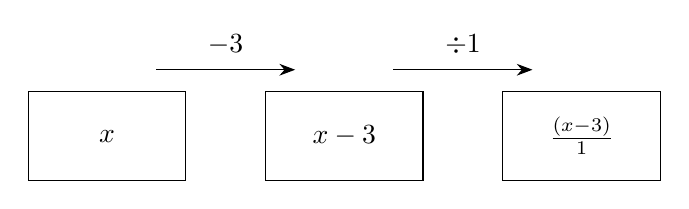
\begin{tikzpicture}[baseline={([yshift=-12pt]current bounding box.north)}]

        \node[backtrack] (boxA) at (0, 0) {$x$};
        \node[backtrack] (boxB) [right=1cm of boxA] {$x-3$};
        \node[backtrack] (boxC) [right=1cm of boxB] {$\frac{(x-3)}{1}$};

        \node (boxAr) at ([yshift=24pt,xshift=5mm]boxA) { };
        \node (boxBl) at ([yshift=24pt,xshift=-5mm]boxB) { };
        \draw [line width=0.4pt,-{Stealth[length=2mm]}] (boxAr)  --node[backtrackstep, above=3.0pt] {$-3$} (boxBl);

        \node (boxBr) at ([yshift=24pt,xshift=5mm]boxB) { };
        \node (boxCl) at ([yshift=24pt,xshift=-5mm]boxC) { };
        \draw [line width=0.4pt,-{Stealth[length=2mm]}] (boxBr)  --node[backtrackstep, above=3.0pt] {$\div1$} (boxCl);

    \end{tikzpicture}
\end{equation}


\vspace{-2pt}\begin{equation}
    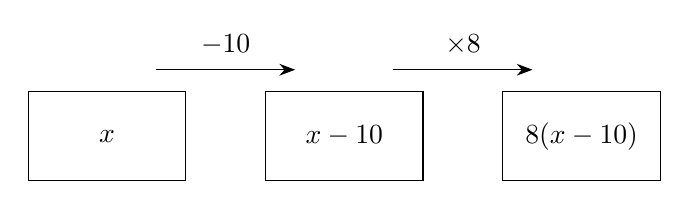
\begin{tikzpicture}[baseline={([yshift=-12pt]current bounding box.north)}]

        \node[backtrack] (boxA) at (0, 0) {$x$};
        \node[backtrack] (boxB) [right=1cm of boxA] {$x-10$};
        \node[backtrack] (boxC) [right=1cm of boxB] {$8(x-10)$};

        \node (boxAr) at ([yshift=24pt,xshift=5mm]boxA) { };
        \node (boxBl) at ([yshift=24pt,xshift=-5mm]boxB) { };
        \draw [line width=0.4pt,-{Stealth[length=2mm]}] (boxAr)  --node[backtrackstep, above=3.0pt] {$-10$} (boxBl);

        \node (boxBr) at ([yshift=24pt,xshift=5mm]boxB) { };
        \node (boxCl) at ([yshift=24pt,xshift=-5mm]boxC) { };
        \draw [line width=0.4pt,-{Stealth[length=2mm]}] (boxBr)  --node[backtrackstep, above=3.0pt] {$\times8$} (boxCl);

    \end{tikzpicture}
\end{equation}


\vspace{-2pt}\begin{equation}
    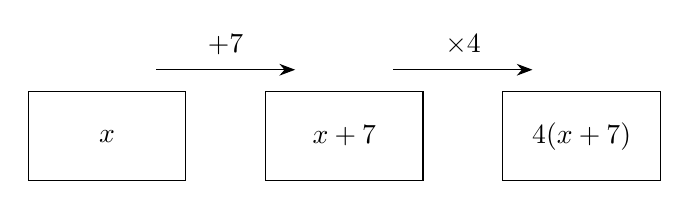
\begin{tikzpicture}[baseline={([yshift=-12pt]current bounding box.north)}]

        \node[backtrack] (boxA) at (0, 0) {$x$};
        \node[backtrack] (boxB) [right=1cm of boxA] {$x+7$};
        \node[backtrack] (boxC) [right=1cm of boxB] {$4(x + 7)$};

        \node (boxAr) at ([yshift=24pt,xshift=5mm]boxA) { };
        \node (boxBl) at ([yshift=24pt,xshift=-5mm]boxB) { };
        \draw [line width=0.4pt,-{Stealth[length=2mm]}] (boxAr)  --node[backtrackstep, above=3.0pt] {$+7$} (boxBl);

        \node (boxBr) at ([yshift=24pt,xshift=5mm]boxB) { };
        \node (boxCl) at ([yshift=24pt,xshift=-5mm]boxC) { };
        \draw [line width=0.4pt,-{Stealth[length=2mm]}] (boxBr)  --node[backtrackstep, above=3.0pt] {$\times4$} (boxCl);

    \end{tikzpicture}
\end{equation}


\vspace{-2pt}\begin{equation}
    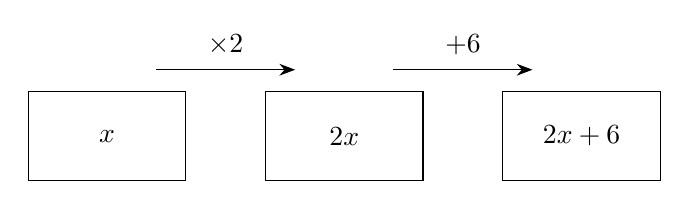
\begin{tikzpicture}[baseline={([yshift=-12pt]current bounding box.north)}]

        \node[backtrack] (boxA) at (0, 0) {$x$};
        \node[backtrack] (boxB) [right=1cm of boxA] {$2x$};
        \node[backtrack] (boxC) [right=1cm of boxB] {$2x + 6$};

        \node (boxAr) at ([yshift=24pt,xshift=5mm]boxA) { };
        \node (boxBl) at ([yshift=24pt,xshift=-5mm]boxB) { };
        \draw [line width=0.4pt,-{Stealth[length=2mm]}] (boxAr)  --node[backtrackstep, above=3.0pt] {$\times2$} (boxBl);

        \node (boxBr) at ([yshift=24pt,xshift=5mm]boxB) { };
        \node (boxCl) at ([yshift=24pt,xshift=-5mm]boxC) { };
        \draw [line width=0.4pt,-{Stealth[length=2mm]}] (boxBr)  --node[backtrackstep, above=3.0pt] {$+6$} (boxCl);

    \end{tikzpicture}
\end{equation}


\vspace{-2pt}\begin{equation}
    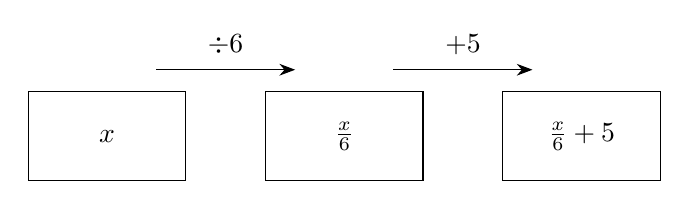
\begin{tikzpicture}[baseline={([yshift=-12pt]current bounding box.north)}]

        \node[backtrack] (boxA) at (0, 0) {$x$};
        \node[backtrack] (boxB) [right=1cm of boxA] {$\frac{x}{6}$};
        \node[backtrack] (boxC) [right=1cm of boxB] {$\frac{x}{6} + 5$};

        \node (boxAr) at ([yshift=24pt,xshift=5mm]boxA) { };
        \node (boxBl) at ([yshift=24pt,xshift=-5mm]boxB) { };
        \draw [line width=0.4pt,-{Stealth[length=2mm]}] (boxAr)  --node[backtrackstep, above=3.0pt] {$\div6$} (boxBl);

        \node (boxBr) at ([yshift=24pt,xshift=5mm]boxB) { };
        \node (boxCl) at ([yshift=24pt,xshift=-5mm]boxC) { };
        \draw [line width=0.4pt,-{Stealth[length=2mm]}] (boxBr)  --node[backtrackstep, above=3.0pt] {$+5$} (boxCl);

    \end{tikzpicture}
\end{equation}


\vspace{-2pt}\begin{equation}
    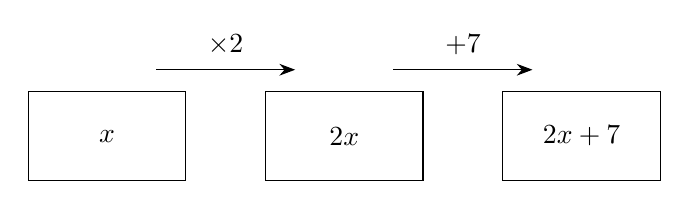
\begin{tikzpicture}[baseline={([yshift=-12pt]current bounding box.north)}]

        \node[backtrack] (boxA) at (0, 0) {$x$};
        \node[backtrack] (boxB) [right=1cm of boxA] {$2x$};
        \node[backtrack] (boxC) [right=1cm of boxB] {$2x + 7$};

        \node (boxAr) at ([yshift=24pt,xshift=5mm]boxA) { };
        \node (boxBl) at ([yshift=24pt,xshift=-5mm]boxB) { };
        \draw [line width=0.4pt,-{Stealth[length=2mm]}] (boxAr)  --node[backtrackstep, above=3.0pt] {$\times2$} (boxBl);

        \node (boxBr) at ([yshift=24pt,xshift=5mm]boxB) { };
        \node (boxCl) at ([yshift=24pt,xshift=-5mm]boxC) { };
        \draw [line width=0.4pt,-{Stealth[length=2mm]}] (boxBr)  --node[backtrackstep, above=3.0pt] {$+7$} (boxCl);

    \end{tikzpicture}
\end{equation}


\vspace{-2pt}\begin{equation}
    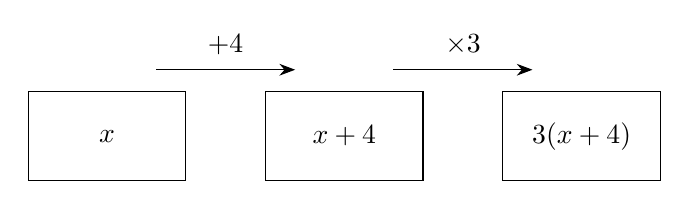
\begin{tikzpicture}[baseline={([yshift=-12pt]current bounding box.north)}]

        \node[backtrack] (boxA) at (0, 0) {$x$};
        \node[backtrack] (boxB) [right=1cm of boxA] {$x+4$};
        \node[backtrack] (boxC) [right=1cm of boxB] {$3(x + 4)$};

        \node (boxAr) at ([yshift=24pt,xshift=5mm]boxA) { };
        \node (boxBl) at ([yshift=24pt,xshift=-5mm]boxB) { };
        \draw [line width=0.4pt,-{Stealth[length=2mm]}] (boxAr)  --node[backtrackstep, above=3.0pt] {$+4$} (boxBl);

        \node (boxBr) at ([yshift=24pt,xshift=5mm]boxB) { };
        \node (boxCl) at ([yshift=24pt,xshift=-5mm]boxC) { };
        \draw [line width=0.4pt,-{Stealth[length=2mm]}] (boxBr)  --node[backtrackstep, above=3.0pt] {$\times3$} (boxCl);

    \end{tikzpicture}
\end{equation}


\vspace{-2pt}\begin{equation}
    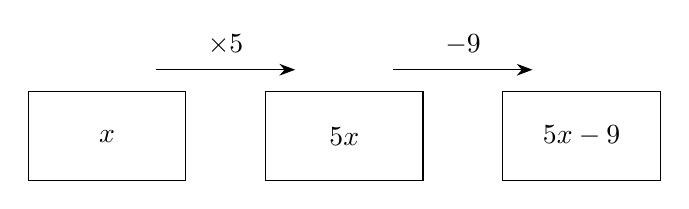
\begin{tikzpicture}[baseline={([yshift=-12pt]current bounding box.north)}]

        \node[backtrack] (boxA) at (0, 0) {$x$};
        \node[backtrack] (boxB) [right=1cm of boxA] {$5x$};
        \node[backtrack] (boxC) [right=1cm of boxB] {$5x - 9$};

        \node (boxAr) at ([yshift=24pt,xshift=5mm]boxA) { };
        \node (boxBl) at ([yshift=24pt,xshift=-5mm]boxB) { };
        \draw [line width=0.4pt,-{Stealth[length=2mm]}] (boxAr)  --node[backtrackstep, above=3.0pt] {$\times5$} (boxBl);

        \node (boxBr) at ([yshift=24pt,xshift=5mm]boxB) { };
        \node (boxCl) at ([yshift=24pt,xshift=-5mm]boxC) { };
        \draw [line width=0.4pt,-{Stealth[length=2mm]}] (boxBr)  --node[backtrackstep, above=3.0pt] {$-9$} (boxCl);

    \end{tikzpicture}
\end{equation}


\vspace{-2pt}\begin{equation}
    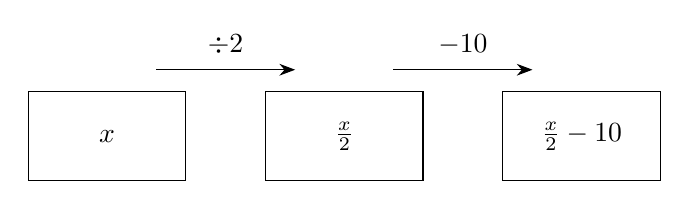
\begin{tikzpicture}[baseline={([yshift=-12pt]current bounding box.north)}]

        \node[backtrack] (boxA) at (0, 0) {$x$};
        \node[backtrack] (boxB) [right=1cm of boxA] {$\frac{x}{2}$};
        \node[backtrack] (boxC) [right=1cm of boxB] {$\frac{x}{2} - 10$};

        \node (boxAr) at ([yshift=24pt,xshift=5mm]boxA) { };
        \node (boxBl) at ([yshift=24pt,xshift=-5mm]boxB) { };
        \draw [line width=0.4pt,-{Stealth[length=2mm]}] (boxAr)  --node[backtrackstep, above=3.0pt] {$\div2$} (boxBl);

        \node (boxBr) at ([yshift=24pt,xshift=5mm]boxB) { };
        \node (boxCl) at ([yshift=24pt,xshift=-5mm]boxC) { };
        \draw [line width=0.4pt,-{Stealth[length=2mm]}] (boxBr)  --node[backtrackstep, above=3.0pt] {$-10$} (boxCl);

    \end{tikzpicture}
\end{equation}


\vspace{-2pt}\begin{equation}
    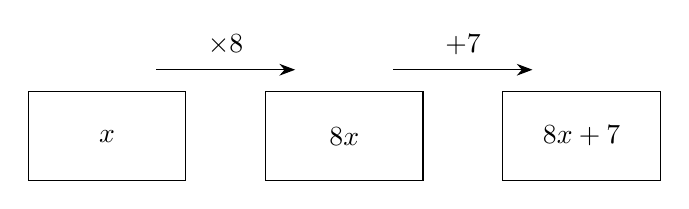
\begin{tikzpicture}[baseline={([yshift=-12pt]current bounding box.north)}]

        \node[backtrack] (boxA) at (0, 0) {$x$};
        \node[backtrack] (boxB) [right=1cm of boxA] {$8x$};
        \node[backtrack] (boxC) [right=1cm of boxB] {$8x + 7$};

        \node (boxAr) at ([yshift=24pt,xshift=5mm]boxA) { };
        \node (boxBl) at ([yshift=24pt,xshift=-5mm]boxB) { };
        \draw [line width=0.4pt,-{Stealth[length=2mm]}] (boxAr)  --node[backtrackstep, above=3.0pt] {$\times8$} (boxBl);

        \node (boxBr) at ([yshift=24pt,xshift=5mm]boxB) { };
        \node (boxCl) at ([yshift=24pt,xshift=-5mm]boxC) { };
        \draw [line width=0.4pt,-{Stealth[length=2mm]}] (boxBr)  --node[backtrackstep, above=3.0pt] {$+7$} (boxCl);

    \end{tikzpicture}
\end{equation}


\vspace{-2pt}\begin{equation}
    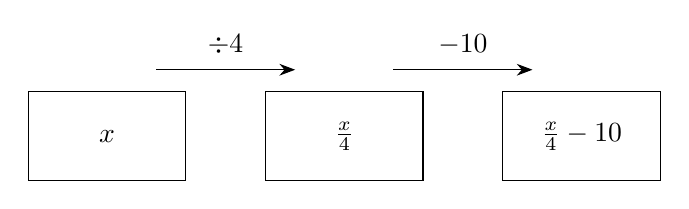
\begin{tikzpicture}[baseline={([yshift=-12pt]current bounding box.north)}]

        \node[backtrack] (boxA) at (0, 0) {$x$};
        \node[backtrack] (boxB) [right=1cm of boxA] {$\frac{x}{4}$};
        \node[backtrack] (boxC) [right=1cm of boxB] {$\frac{x}{4} - 10$};

        \node (boxAr) at ([yshift=24pt,xshift=5mm]boxA) { };
        \node (boxBl) at ([yshift=24pt,xshift=-5mm]boxB) { };
        \draw [line width=0.4pt,-{Stealth[length=2mm]}] (boxAr)  --node[backtrackstep, above=3.0pt] {$\div4$} (boxBl);

        \node (boxBr) at ([yshift=24pt,xshift=5mm]boxB) { };
        \node (boxCl) at ([yshift=24pt,xshift=-5mm]boxC) { };
        \draw [line width=0.4pt,-{Stealth[length=2mm]}] (boxBr)  --node[backtrackstep, above=3.0pt] {$-10$} (boxCl);

    \end{tikzpicture}
\end{equation}


\vspace{-2pt}\begin{equation}
    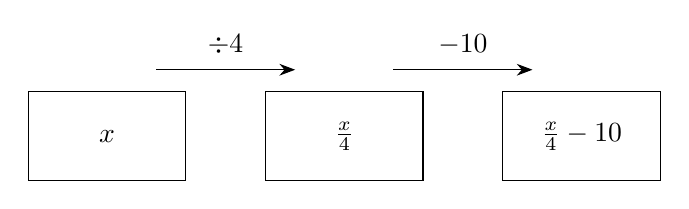
\begin{tikzpicture}[baseline={([yshift=-12pt]current bounding box.north)}]

        \node[backtrack] (boxA) at (0, 0) {$x$};
        \node[backtrack] (boxB) [right=1cm of boxA] {$\frac{x}{4}$};
        \node[backtrack] (boxC) [right=1cm of boxB] {$\frac{x}{4} - 10$};

        \node (boxAr) at ([yshift=24pt,xshift=5mm]boxA) { };
        \node (boxBl) at ([yshift=24pt,xshift=-5mm]boxB) { };
        \draw [line width=0.4pt,-{Stealth[length=2mm]}] (boxAr)  --node[backtrackstep, above=3.0pt] {$\div4$} (boxBl);

        \node (boxBr) at ([yshift=24pt,xshift=5mm]boxB) { };
        \node (boxCl) at ([yshift=24pt,xshift=-5mm]boxC) { };
        \draw [line width=0.4pt,-{Stealth[length=2mm]}] (boxBr)  --node[backtrackstep, above=3.0pt] {$-10$} (boxCl);

    \end{tikzpicture}
\end{equation}


\vspace{-2pt}\begin{equation}
    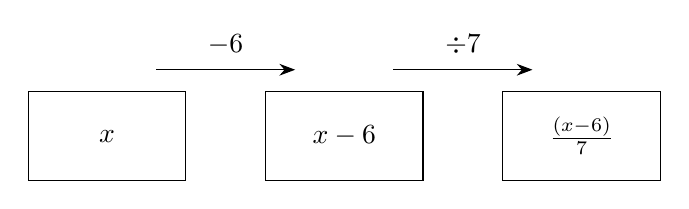
\begin{tikzpicture}[baseline={([yshift=-12pt]current bounding box.north)}]

        \node[backtrack] (boxA) at (0, 0) {$x$};
        \node[backtrack] (boxB) [right=1cm of boxA] {$x-6$};
        \node[backtrack] (boxC) [right=1cm of boxB] {$\frac{(x-6)}{7}$};

        \node (boxAr) at ([yshift=24pt,xshift=5mm]boxA) { };
        \node (boxBl) at ([yshift=24pt,xshift=-5mm]boxB) { };
        \draw [line width=0.4pt,-{Stealth[length=2mm]}] (boxAr)  --node[backtrackstep, above=3.0pt] {$-6$} (boxBl);

        \node (boxBr) at ([yshift=24pt,xshift=5mm]boxB) { };
        \node (boxCl) at ([yshift=24pt,xshift=-5mm]boxC) { };
        \draw [line width=0.4pt,-{Stealth[length=2mm]}] (boxBr)  --node[backtrackstep, above=3.0pt] {$\div7$} (boxCl);

    \end{tikzpicture}
\end{equation}


\vspace{-2pt}\begin{equation}
    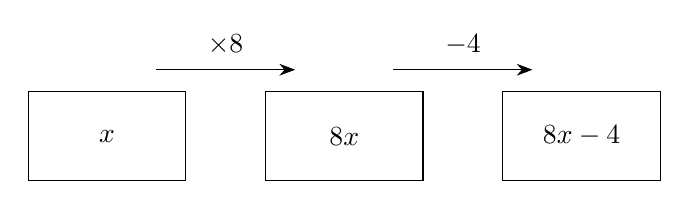
\begin{tikzpicture}[baseline={([yshift=-12pt]current bounding box.north)}]

        \node[backtrack] (boxA) at (0, 0) {$x$};
        \node[backtrack] (boxB) [right=1cm of boxA] {$8x$};
        \node[backtrack] (boxC) [right=1cm of boxB] {$8x - 4$};

        \node (boxAr) at ([yshift=24pt,xshift=5mm]boxA) { };
        \node (boxBl) at ([yshift=24pt,xshift=-5mm]boxB) { };
        \draw [line width=0.4pt,-{Stealth[length=2mm]}] (boxAr)  --node[backtrackstep, above=3.0pt] {$\times8$} (boxBl);

        \node (boxBr) at ([yshift=24pt,xshift=5mm]boxB) { };
        \node (boxCl) at ([yshift=24pt,xshift=-5mm]boxC) { };
        \draw [line width=0.4pt,-{Stealth[length=2mm]}] (boxBr)  --node[backtrackstep, above=3.0pt] {$-4$} (boxCl);

    \end{tikzpicture}
\end{equation}


\vspace{-2pt}\begin{equation}
    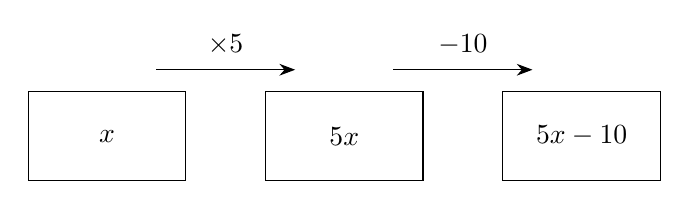
\begin{tikzpicture}[baseline={([yshift=-12pt]current bounding box.north)}]

        \node[backtrack] (boxA) at (0, 0) {$x$};
        \node[backtrack] (boxB) [right=1cm of boxA] {$5x$};
        \node[backtrack] (boxC) [right=1cm of boxB] {$5x - 10$};

        \node (boxAr) at ([yshift=24pt,xshift=5mm]boxA) { };
        \node (boxBl) at ([yshift=24pt,xshift=-5mm]boxB) { };
        \draw [line width=0.4pt,-{Stealth[length=2mm]}] (boxAr)  --node[backtrackstep, above=3.0pt] {$\times5$} (boxBl);

        \node (boxBr) at ([yshift=24pt,xshift=5mm]boxB) { };
        \node (boxCl) at ([yshift=24pt,xshift=-5mm]boxC) { };
        \draw [line width=0.4pt,-{Stealth[length=2mm]}] (boxBr)  --node[backtrackstep, above=3.0pt] {$-10$} (boxCl);

    \end{tikzpicture}
\end{equation}


\vspace{-2pt}\begin{equation}
    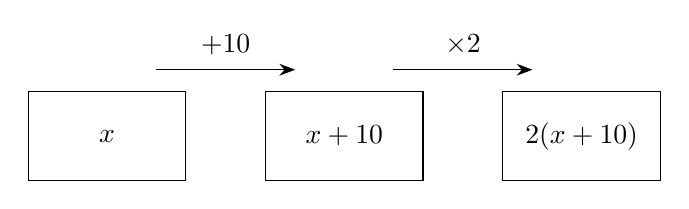
\begin{tikzpicture}[baseline={([yshift=-12pt]current bounding box.north)}]

        \node[backtrack] (boxA) at (0, 0) {$x$};
        \node[backtrack] (boxB) [right=1cm of boxA] {$x+10$};
        \node[backtrack] (boxC) [right=1cm of boxB] {$2(x + 10)$};

        \node (boxAr) at ([yshift=24pt,xshift=5mm]boxA) { };
        \node (boxBl) at ([yshift=24pt,xshift=-5mm]boxB) { };
        \draw [line width=0.4pt,-{Stealth[length=2mm]}] (boxAr)  --node[backtrackstep, above=3.0pt] {$+10$} (boxBl);

        \node (boxBr) at ([yshift=24pt,xshift=5mm]boxB) { };
        \node (boxCl) at ([yshift=24pt,xshift=-5mm]boxC) { };
        \draw [line width=0.4pt,-{Stealth[length=2mm]}] (boxBr)  --node[backtrackstep, above=3.0pt] {$\times2$} (boxCl);

    \end{tikzpicture}
\end{equation}


\vspace{-2pt}\begin{equation}
    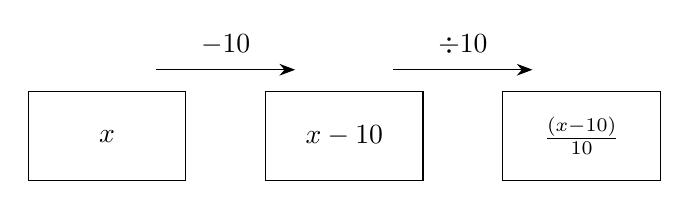
\begin{tikzpicture}[baseline={([yshift=-12pt]current bounding box.north)}]

        \node[backtrack] (boxA) at (0, 0) {$x$};
        \node[backtrack] (boxB) [right=1cm of boxA] {$x-10$};
        \node[backtrack] (boxC) [right=1cm of boxB] {$\frac{(x-10)}{10}$};

        \node (boxAr) at ([yshift=24pt,xshift=5mm]boxA) { };
        \node (boxBl) at ([yshift=24pt,xshift=-5mm]boxB) { };
        \draw [line width=0.4pt,-{Stealth[length=2mm]}] (boxAr)  --node[backtrackstep, above=3.0pt] {$-10$} (boxBl);

        \node (boxBr) at ([yshift=24pt,xshift=5mm]boxB) { };
        \node (boxCl) at ([yshift=24pt,xshift=-5mm]boxC) { };
        \draw [line width=0.4pt,-{Stealth[length=2mm]}] (boxBr)  --node[backtrackstep, above=3.0pt] {$\div10$} (boxCl);

    \end{tikzpicture}
\end{equation}


\vspace{-2pt}\begin{equation}
    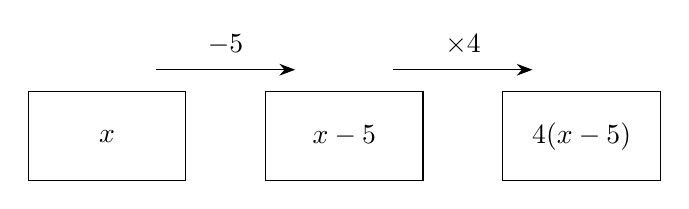
\begin{tikzpicture}[baseline={([yshift=-12pt]current bounding box.north)}]

        \node[backtrack] (boxA) at (0, 0) {$x$};
        \node[backtrack] (boxB) [right=1cm of boxA] {$x-5$};
        \node[backtrack] (boxC) [right=1cm of boxB] {$4(x-5)$};

        \node (boxAr) at ([yshift=24pt,xshift=5mm]boxA) { };
        \node (boxBl) at ([yshift=24pt,xshift=-5mm]boxB) { };
        \draw [line width=0.4pt,-{Stealth[length=2mm]}] (boxAr)  --node[backtrackstep, above=3.0pt] {$-5$} (boxBl);

        \node (boxBr) at ([yshift=24pt,xshift=5mm]boxB) { };
        \node (boxCl) at ([yshift=24pt,xshift=-5mm]boxC) { };
        \draw [line width=0.4pt,-{Stealth[length=2mm]}] (boxBr)  --node[backtrackstep, above=3.0pt] {$\times4$} (boxCl);

    \end{tikzpicture}
\end{equation}


\vspace{-2pt}\begin{equation}
    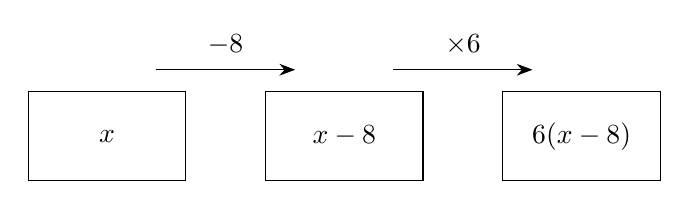
\begin{tikzpicture}[baseline={([yshift=-12pt]current bounding box.north)}]

        \node[backtrack] (boxA) at (0, 0) {$x$};
        \node[backtrack] (boxB) [right=1cm of boxA] {$x-8$};
        \node[backtrack] (boxC) [right=1cm of boxB] {$6(x-8)$};

        \node (boxAr) at ([yshift=24pt,xshift=5mm]boxA) { };
        \node (boxBl) at ([yshift=24pt,xshift=-5mm]boxB) { };
        \draw [line width=0.4pt,-{Stealth[length=2mm]}] (boxAr)  --node[backtrackstep, above=3.0pt] {$-8$} (boxBl);

        \node (boxBr) at ([yshift=24pt,xshift=5mm]boxB) { };
        \node (boxCl) at ([yshift=24pt,xshift=-5mm]boxC) { };
        \draw [line width=0.4pt,-{Stealth[length=2mm]}] (boxBr)  --node[backtrackstep, above=3.0pt] {$\times6$} (boxCl);

    \end{tikzpicture}
\end{equation}


\vspace{-2pt}\begin{equation}
    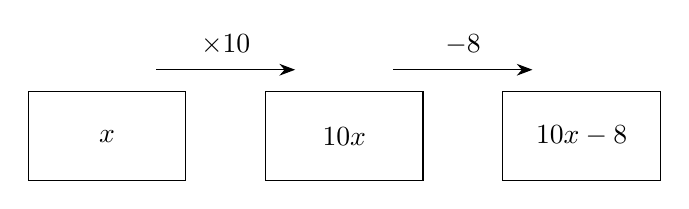
\begin{tikzpicture}[baseline={([yshift=-12pt]current bounding box.north)}]

        \node[backtrack] (boxA) at (0, 0) {$x$};
        \node[backtrack] (boxB) [right=1cm of boxA] {$10x$};
        \node[backtrack] (boxC) [right=1cm of boxB] {$10x - 8$};

        \node (boxAr) at ([yshift=24pt,xshift=5mm]boxA) { };
        \node (boxBl) at ([yshift=24pt,xshift=-5mm]boxB) { };
        \draw [line width=0.4pt,-{Stealth[length=2mm]}] (boxAr)  --node[backtrackstep, above=3.0pt] {$\times10$} (boxBl);

        \node (boxBr) at ([yshift=24pt,xshift=5mm]boxB) { };
        \node (boxCl) at ([yshift=24pt,xshift=-5mm]boxC) { };
        \draw [line width=0.4pt,-{Stealth[length=2mm]}] (boxBr)  --node[backtrackstep, above=3.0pt] {$-8$} (boxCl);

    \end{tikzpicture}
\end{equation}


\vspace{-2pt}\begin{equation}
    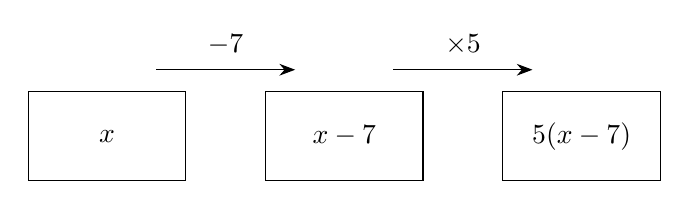
\begin{tikzpicture}[baseline={([yshift=-12pt]current bounding box.north)}]

        \node[backtrack] (boxA) at (0, 0) {$x$};
        \node[backtrack] (boxB) [right=1cm of boxA] {$x-7$};
        \node[backtrack] (boxC) [right=1cm of boxB] {$5(x-7)$};

        \node (boxAr) at ([yshift=24pt,xshift=5mm]boxA) { };
        \node (boxBl) at ([yshift=24pt,xshift=-5mm]boxB) { };
        \draw [line width=0.4pt,-{Stealth[length=2mm]}] (boxAr)  --node[backtrackstep, above=3.0pt] {$-7$} (boxBl);

        \node (boxBr) at ([yshift=24pt,xshift=5mm]boxB) { };
        \node (boxCl) at ([yshift=24pt,xshift=-5mm]boxC) { };
        \draw [line width=0.4pt,-{Stealth[length=2mm]}] (boxBr)  --node[backtrackstep, above=3.0pt] {$\times5$} (boxCl);

    \end{tikzpicture}
\end{equation}


\vspace{-2pt}\begin{equation}
    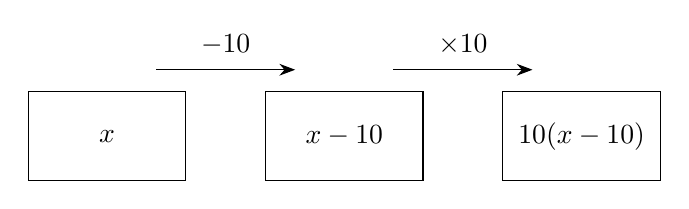
\begin{tikzpicture}[baseline={([yshift=-12pt]current bounding box.north)}]

        \node[backtrack] (boxA) at (0, 0) {$x$};
        \node[backtrack] (boxB) [right=1cm of boxA] {$x-10$};
        \node[backtrack] (boxC) [right=1cm of boxB] {$10(x-10)$};

        \node (boxAr) at ([yshift=24pt,xshift=5mm]boxA) { };
        \node (boxBl) at ([yshift=24pt,xshift=-5mm]boxB) { };
        \draw [line width=0.4pt,-{Stealth[length=2mm]}] (boxAr)  --node[backtrackstep, above=3.0pt] {$-10$} (boxBl);

        \node (boxBr) at ([yshift=24pt,xshift=5mm]boxB) { };
        \node (boxCl) at ([yshift=24pt,xshift=-5mm]boxC) { };
        \draw [line width=0.4pt,-{Stealth[length=2mm]}] (boxBr)  --node[backtrackstep, above=3.0pt] {$\times10$} (boxCl);

    \end{tikzpicture}
\end{equation}


\vspace{-2pt}\begin{equation}
    \begin{tikzpicture}[baseline={([yshift=-12pt]current bounding box.north)}]

        \node[backtrack] (boxA) at (0, 0) {$x$};
        \node[backtrack] (boxB) [right=1cm of boxA] {$\frac{x}{4}$};
        \node[backtrack] (boxC) [right=1cm of boxB] {$\frac{x}{4} - 2$};

        \node (boxAr) at ([yshift=24pt,xshift=5mm]boxA) { };
        \node (boxBl) at ([yshift=24pt,xshift=-5mm]boxB) { };
        \draw [line width=0.4pt,-{Stealth[length=2mm]}] (boxAr)  --node[backtrackstep, above=3.0pt] {$\div4$} (boxBl);

        \node (boxBr) at ([yshift=24pt,xshift=5mm]boxB) { };
        \node (boxCl) at ([yshift=24pt,xshift=-5mm]boxC) { };
        \draw [line width=0.4pt,-{Stealth[length=2mm]}] (boxBr)  --node[backtrackstep, above=3.0pt] {$-2$} (boxCl);

    \end{tikzpicture}
\end{equation}


\vspace{-2pt}\begin{equation}
    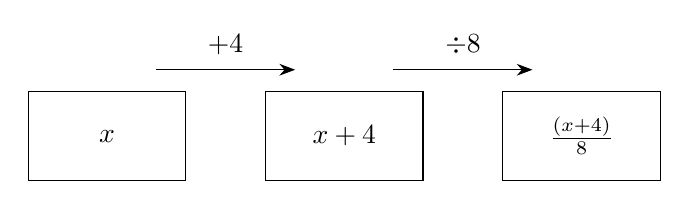
\begin{tikzpicture}[baseline={([yshift=-12pt]current bounding box.north)}]

        \node[backtrack] (boxA) at (0, 0) {$x$};
        \node[backtrack] (boxB) [right=1cm of boxA] {$x+4$};
        \node[backtrack] (boxC) [right=1cm of boxB] {$\frac{(x+4)}{8}$};

        \node (boxAr) at ([yshift=24pt,xshift=5mm]boxA) { };
        \node (boxBl) at ([yshift=24pt,xshift=-5mm]boxB) { };
        \draw [line width=0.4pt,-{Stealth[length=2mm]}] (boxAr)  --node[backtrackstep, above=3.0pt] {$+4$} (boxBl);

        \node (boxBr) at ([yshift=24pt,xshift=5mm]boxB) { };
        \node (boxCl) at ([yshift=24pt,xshift=-5mm]boxC) { };
        \draw [line width=0.4pt,-{Stealth[length=2mm]}] (boxBr)  --node[backtrackstep, above=3.0pt] {$\div8$} (boxCl);

    \end{tikzpicture}
\end{equation}


\vspace{-2pt}\begin{equation}
    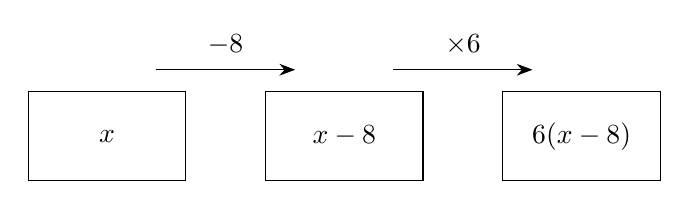
\begin{tikzpicture}[baseline={([yshift=-12pt]current bounding box.north)}]

        \node[backtrack] (boxA) at (0, 0) {$x$};
        \node[backtrack] (boxB) [right=1cm of boxA] {$x-8$};
        \node[backtrack] (boxC) [right=1cm of boxB] {$6(x-8)$};

        \node (boxAr) at ([yshift=24pt,xshift=5mm]boxA) { };
        \node (boxBl) at ([yshift=24pt,xshift=-5mm]boxB) { };
        \draw [line width=0.4pt,-{Stealth[length=2mm]}] (boxAr)  --node[backtrackstep, above=3.0pt] {$-8$} (boxBl);

        \node (boxBr) at ([yshift=24pt,xshift=5mm]boxB) { };
        \node (boxCl) at ([yshift=24pt,xshift=-5mm]boxC) { };
        \draw [line width=0.4pt,-{Stealth[length=2mm]}] (boxBr)  --node[backtrackstep, above=3.0pt] {$\times6$} (boxCl);

    \end{tikzpicture}
\end{equation}


\vspace{-2pt}\begin{equation}
    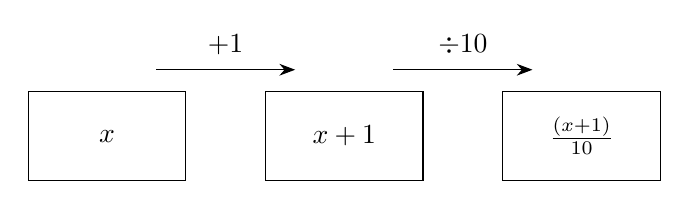
\begin{tikzpicture}[baseline={([yshift=-12pt]current bounding box.north)}]

        \node[backtrack] (boxA) at (0, 0) {$x$};
        \node[backtrack] (boxB) [right=1cm of boxA] {$x+1$};
        \node[backtrack] (boxC) [right=1cm of boxB] {$\frac{(x+1)}{10}$};

        \node (boxAr) at ([yshift=24pt,xshift=5mm]boxA) { };
        \node (boxBl) at ([yshift=24pt,xshift=-5mm]boxB) { };
        \draw [line width=0.4pt,-{Stealth[length=2mm]}] (boxAr)  --node[backtrackstep, above=3.0pt] {$+1$} (boxBl);

        \node (boxBr) at ([yshift=24pt,xshift=5mm]boxB) { };
        \node (boxCl) at ([yshift=24pt,xshift=-5mm]boxC) { };
        \draw [line width=0.4pt,-{Stealth[length=2mm]}] (boxBr)  --node[backtrackstep, above=3.0pt] {$\div10$} (boxCl);

    \end{tikzpicture}
\end{equation}


\vspace{-2pt}\begin{equation}
    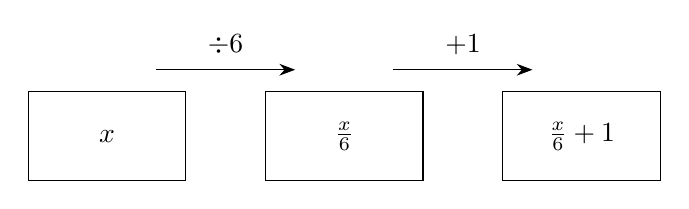
\begin{tikzpicture}[baseline={([yshift=-12pt]current bounding box.north)}]

        \node[backtrack] (boxA) at (0, 0) {$x$};
        \node[backtrack] (boxB) [right=1cm of boxA] {$\frac{x}{6}$};
        \node[backtrack] (boxC) [right=1cm of boxB] {$\frac{x}{6} + 1$};

        \node (boxAr) at ([yshift=24pt,xshift=5mm]boxA) { };
        \node (boxBl) at ([yshift=24pt,xshift=-5mm]boxB) { };
        \draw [line width=0.4pt,-{Stealth[length=2mm]}] (boxAr)  --node[backtrackstep, above=3.0pt] {$\div6$} (boxBl);

        \node (boxBr) at ([yshift=24pt,xshift=5mm]boxB) { };
        \node (boxCl) at ([yshift=24pt,xshift=-5mm]boxC) { };
        \draw [line width=0.4pt,-{Stealth[length=2mm]}] (boxBr)  --node[backtrackstep, above=3.0pt] {$+1$} (boxCl);

    \end{tikzpicture}
\end{equation}


\vspace{-2pt}\begin{equation}
    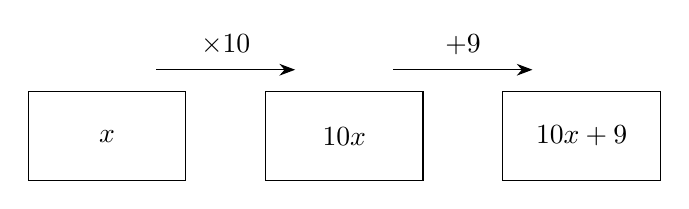
\begin{tikzpicture}[baseline={([yshift=-12pt]current bounding box.north)}]

        \node[backtrack] (boxA) at (0, 0) {$x$};
        \node[backtrack] (boxB) [right=1cm of boxA] {$10x$};
        \node[backtrack] (boxC) [right=1cm of boxB] {$10x + 9$};

        \node (boxAr) at ([yshift=24pt,xshift=5mm]boxA) { };
        \node (boxBl) at ([yshift=24pt,xshift=-5mm]boxB) { };
        \draw [line width=0.4pt,-{Stealth[length=2mm]}] (boxAr)  --node[backtrackstep, above=3.0pt] {$\times10$} (boxBl);

        \node (boxBr) at ([yshift=24pt,xshift=5mm]boxB) { };
        \node (boxCl) at ([yshift=24pt,xshift=-5mm]boxC) { };
        \draw [line width=0.4pt,-{Stealth[length=2mm]}] (boxBr)  --node[backtrackstep, above=3.0pt] {$+9$} (boxCl);

    \end{tikzpicture}
\end{equation}


\vspace{-2pt}\begin{equation}
    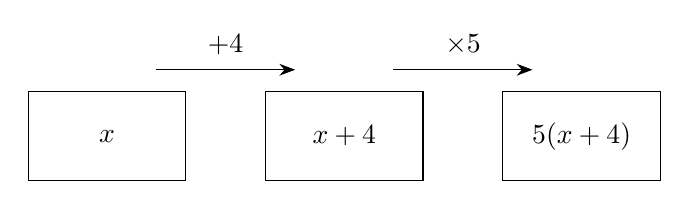
\begin{tikzpicture}[baseline={([yshift=-12pt]current bounding box.north)}]

        \node[backtrack] (boxA) at (0, 0) {$x$};
        \node[backtrack] (boxB) [right=1cm of boxA] {$x+4$};
        \node[backtrack] (boxC) [right=1cm of boxB] {$5(x + 4)$};

        \node (boxAr) at ([yshift=24pt,xshift=5mm]boxA) { };
        \node (boxBl) at ([yshift=24pt,xshift=-5mm]boxB) { };
        \draw [line width=0.4pt,-{Stealth[length=2mm]}] (boxAr)  --node[backtrackstep, above=3.0pt] {$+4$} (boxBl);

        \node (boxBr) at ([yshift=24pt,xshift=5mm]boxB) { };
        \node (boxCl) at ([yshift=24pt,xshift=-5mm]boxC) { };
        \draw [line width=0.4pt,-{Stealth[length=2mm]}] (boxBr)  --node[backtrackstep, above=3.0pt] {$\times5$} (boxCl);

    \end{tikzpicture}
\end{equation}


\vspace{-2pt}\begin{equation}
    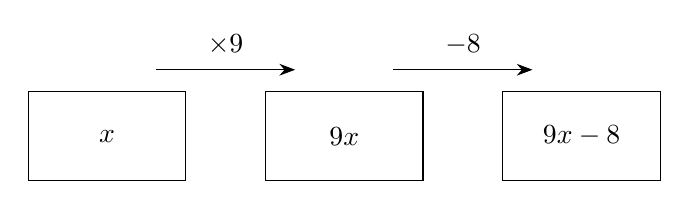
\begin{tikzpicture}[baseline={([yshift=-12pt]current bounding box.north)}]

        \node[backtrack] (boxA) at (0, 0) {$x$};
        \node[backtrack] (boxB) [right=1cm of boxA] {$9x$};
        \node[backtrack] (boxC) [right=1cm of boxB] {$9x - 8$};

        \node (boxAr) at ([yshift=24pt,xshift=5mm]boxA) { };
        \node (boxBl) at ([yshift=24pt,xshift=-5mm]boxB) { };
        \draw [line width=0.4pt,-{Stealth[length=2mm]}] (boxAr)  --node[backtrackstep, above=3.0pt] {$\times9$} (boxBl);

        \node (boxBr) at ([yshift=24pt,xshift=5mm]boxB) { };
        \node (boxCl) at ([yshift=24pt,xshift=-5mm]boxC) { };
        \draw [line width=0.4pt,-{Stealth[length=2mm]}] (boxBr)  --node[backtrackstep, above=3.0pt] {$-8$} (boxCl);

    \end{tikzpicture}
\end{equation}


\vspace{-2pt}\begin{equation}
    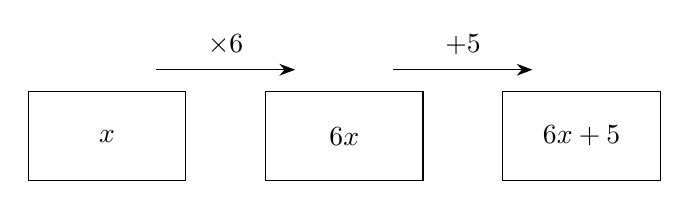
\begin{tikzpicture}[baseline={([yshift=-12pt]current bounding box.north)}]

        \node[backtrack] (boxA) at (0, 0) {$x$};
        \node[backtrack] (boxB) [right=1cm of boxA] {$6x$};
        \node[backtrack] (boxC) [right=1cm of boxB] {$6x + 5$};

        \node (boxAr) at ([yshift=24pt,xshift=5mm]boxA) { };
        \node (boxBl) at ([yshift=24pt,xshift=-5mm]boxB) { };
        \draw [line width=0.4pt,-{Stealth[length=2mm]}] (boxAr)  --node[backtrackstep, above=3.0pt] {$\times6$} (boxBl);

        \node (boxBr) at ([yshift=24pt,xshift=5mm]boxB) { };
        \node (boxCl) at ([yshift=24pt,xshift=-5mm]boxC) { };
        \draw [line width=0.4pt,-{Stealth[length=2mm]}] (boxBr)  --node[backtrackstep, above=3.0pt] {$+5$} (boxCl);

    \end{tikzpicture}
\end{equation}


\vspace{-2pt}\begin{equation}
    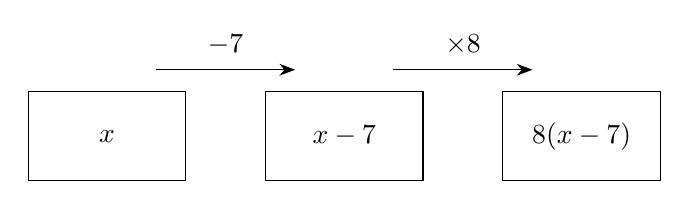
\begin{tikzpicture}[baseline={([yshift=-12pt]current bounding box.north)}]

        \node[backtrack] (boxA) at (0, 0) {$x$};
        \node[backtrack] (boxB) [right=1cm of boxA] {$x-7$};
        \node[backtrack] (boxC) [right=1cm of boxB] {$8(x-7)$};

        \node (boxAr) at ([yshift=24pt,xshift=5mm]boxA) { };
        \node (boxBl) at ([yshift=24pt,xshift=-5mm]boxB) { };
        \draw [line width=0.4pt,-{Stealth[length=2mm]}] (boxAr)  --node[backtrackstep, above=3.0pt] {$-7$} (boxBl);

        \node (boxBr) at ([yshift=24pt,xshift=5mm]boxB) { };
        \node (boxCl) at ([yshift=24pt,xshift=-5mm]boxC) { };
        \draw [line width=0.4pt,-{Stealth[length=2mm]}] (boxBr)  --node[backtrackstep, above=3.0pt] {$\times8$} (boxCl);

    \end{tikzpicture}
\end{equation}


\vspace{-2pt}\begin{equation}
    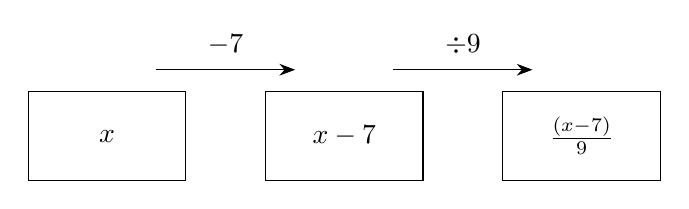
\begin{tikzpicture}[baseline={([yshift=-12pt]current bounding box.north)}]

        \node[backtrack] (boxA) at (0, 0) {$x$};
        \node[backtrack] (boxB) [right=1cm of boxA] {$x-7$};
        \node[backtrack] (boxC) [right=1cm of boxB] {$\frac{(x-7)}{9}$};

        \node (boxAr) at ([yshift=24pt,xshift=5mm]boxA) { };
        \node (boxBl) at ([yshift=24pt,xshift=-5mm]boxB) { };
        \draw [line width=0.4pt,-{Stealth[length=2mm]}] (boxAr)  --node[backtrackstep, above=3.0pt] {$-7$} (boxBl);

        \node (boxBr) at ([yshift=24pt,xshift=5mm]boxB) { };
        \node (boxCl) at ([yshift=24pt,xshift=-5mm]boxC) { };
        \draw [line width=0.4pt,-{Stealth[length=2mm]}] (boxBr)  --node[backtrackstep, above=3.0pt] {$\div9$} (boxCl);

    \end{tikzpicture}
\end{equation}


\vspace{-2pt}\begin{equation}
    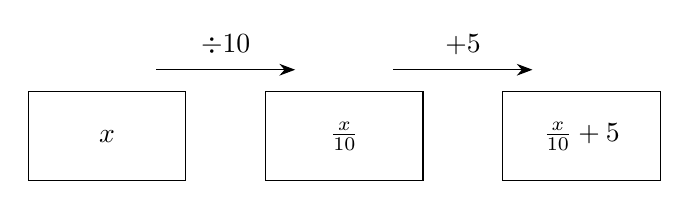
\begin{tikzpicture}[baseline={([yshift=-12pt]current bounding box.north)}]

        \node[backtrack] (boxA) at (0, 0) {$x$};
        \node[backtrack] (boxB) [right=1cm of boxA] {$\frac{x}{10}$};
        \node[backtrack] (boxC) [right=1cm of boxB] {$\frac{x}{10} + 5$};

        \node (boxAr) at ([yshift=24pt,xshift=5mm]boxA) { };
        \node (boxBl) at ([yshift=24pt,xshift=-5mm]boxB) { };
        \draw [line width=0.4pt,-{Stealth[length=2mm]}] (boxAr)  --node[backtrackstep, above=3.0pt] {$\div10$} (boxBl);

        \node (boxBr) at ([yshift=24pt,xshift=5mm]boxB) { };
        \node (boxCl) at ([yshift=24pt,xshift=-5mm]boxC) { };
        \draw [line width=0.4pt,-{Stealth[length=2mm]}] (boxBr)  --node[backtrackstep, above=3.0pt] {$+5$} (boxCl);

    \end{tikzpicture}
\end{equation}


\vspace{-2pt}
    \end{multicols}
\end{document}
